\documentclass{article}
\usepackage{array}
\usepackage[T1]{fontenc}
\usepackage[Russian]{babel}
\usepackage{booktabs}
\usepackage{graphicx}
\begin{document}
\author{Осипов Александр Б06-604}
\title{Лабораторная работа 1.1.1. Определение систематических и случайных погрешностей при измерении удельного сопротивления нихромовой проволки}
\maketitle
\section{Цель}

Измерить удельное сопротивлене проволки и вычислить систематические и случаные погрешности.

\section{Оборудование} 

Вольметр, амперметр, штангенциркуль, микрометр, линейка
проволка из нихрома, источник ЭДС, мост постоянного тока
\section {Теоретическая часть}
\section{Ход работы}
 
\vspace{0.5cm} 

d1 - микрометр
d2 - штангенциркуль

\textbf{\large Таблица 1 - результаты измерения диаметра проволки}
 
\vspace{0.5cm}

\begin{tabular}{ccccccccccc}
     &1&2&3&4&5&6&7&8&9&10\\ 
    d1, mm & 0.34 & 0.35 & 0.36 & 0.36 & 0.37 & 0.36 & 0.36 & 0.36\\
    d2, mm & 0.4 & 0.4 & 0.4 & 0.4 & 0.4 & 0.4 & 0.4 & 0.4\\
\end{tabular}

\vspace{0.5cm}
Расчет случайной ошибки при измерении штангенциркулем:

Расчет случайной ошибки при измерении микрометром:
\vspace{0.5cm}

\textbf{\large Таблица 2 - Основные характеристики приборов}

\begin{tabular}{ccc}
     & Вольтметр & Миллиамперметр\\
    Система & &\\
    Класс точности & & \\
    ...\\
    Внутреннее сопротивление прибора \\
\end{tabular}

\vspace{5mm}

Оценка ошибки при измерении схемой а и б:

\vspace{5mm}

\textbf{\large Таблица 3 - Показания вольтметра и амперметра}

Вольтметр 150 делений максимум 750 мВ


\begin{tabular}{ccccccccccccc}
    \multicolumn{4}{c}{l = 20 см} |& \multicolumn{4}{c}{l = 30 см} |& \multicolumn{4}{c}{l = 50 см}\\ 
     & V,дел & I,дел & V,мВ & I, мА | & V,дел & I,дел & V,мВ & I, мА | & V,дел & I,дел & V,мВ & I, мА\\
    \toprule 
    1 & 147 & 358.8 & f & 358.8 |  & 149 & 245.7 & f & 245.7 | & 150 & 148.2 & f & 148.2\\
    \midrule
    2 & 136 & 333.4 & f & 333.4 | & 123 & 203.0 & f & 203.0 | & 131 & 129.9 & f & 129.9\\
    \midrule
    3 & 117 & 286.2 & f & 286.2 | & 101 & 174.9 & f & 174.9 | & 124 & 122.2 & f & 122.2\\
    \midrule
    4 & 98 & 239.2 & f & 239.5 | & 95 & 156.7 & f & 156.7 | & 109 & 107.9 & f & 107.9\\
    \midrule
    5 & 79 & 191.5 & f & 191.5 | & 83 & 136.7 & f & 136.7 | & 95 & 094.2 & f & 094.2\\
    \midrule
    6 & 67 & 164.1 & f & 164.1 | & 66 & 109.0 & f & 109.0 | & 87 & 085.7 & f & 085.7\\
    \midrule
    7 & 59 & 131.5 & f & 131.5 | & 50 & 083.3 & f & 083.3 | & 82 & 081.0 & f & 081.0\\
    \midrule
    8 & 43 & 106.3 & f & 106.3 | & 45 & 075.2 & f & 075.2 | & 75 & 074.6 & f & 074.6\\
    \midrule
    9 & 30 & 073.6 & f & 073.6 | & 42 & 069.6 & f & 069.9 | & 69 & 068.4 & f & 068.4\\
    \midrule
    10 & 26 & 065.3 & f & 065.3 | & 39 & 064.1 & f & 064.1 | & 62 & 061.7 & f & 061.7\\
    \midrule
\end{tabular}

\vspace{5mm}

Замеры на мосте 

20 см

2.1797

30cv 

3.1669

50

5.2225 Ом

погрешность 0.5 процента * 750 mv

у электронного прибора точность измерения последняя цифра которая не дрожит

\textbf{\large Таблица 4 - Результаты измерения сопротивления проволки}


\begin{tabular}{ccc}
    l = 20 мм& l = 30см & l = 50 см\\
     & &\\
     & & \\
    ...\\
\end{tabular}

\textbf{\large Таблица 6 - Результаты расчета удельного сопротивления проволки}


\begin{tabular}{ccc}
    l, см & $\rho, 10^{-4}$ Ом*см& $\rho, 10^{-6} Ом*см$ \\
     & &\\
     & & \\
    ...\\
\end{tabular}


\begin{center}
  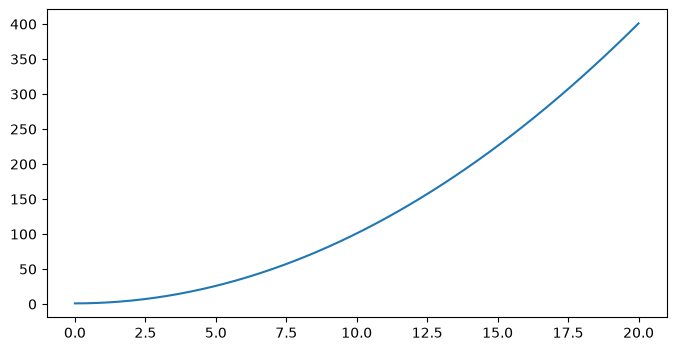
\includegraphics[height=2cm]{plot.png}
\end{center}


\end{document}